\chapter{Conceito do Sistema}
\label{chap:concep}
%\begin{flushright}
%   \begin{list}{}{
%      \setlength{\leftmargin}{4.5cm}
%      \setlength{\rightmargin}{0cm}
%      \setlength{\labelwidth}{0pt}
%      \setlength{\labelsep}{\leftmargin}}
%      \item Quanto maior for a rapidez de transformação de uma
%      sociedade, mais temporárias são as necessidades
%      individuais. Essas flutuaçõess tornam ainda mais acelerado
%      o senso de turbilh da sociedade.
%
%      \begin{list}{}{
%      \setlength{\leftmargin}{0cm}
%      \setlength{\rightmargin}{0cm}
%      \setlength{\labelwidth}{0pt}
%      \setlength{\labelsep}{\leftmargin}}
%      \item (Alvin Toffler)
%      \end{list}
%   \end{list}
%\end{flushright}

\begin{flushright}
  Nada é tão maravilhoso que não possa existir, \\
  se admitido pelas leis da Natureza. \\
  \ \\
  (Michael Faraday)
\end{flushright}



%--------- NEW SECTION ----------------------
\section{Estudo do estado da arte}
\label{sec:sota}
Diante dos desafios apresentados nesta tese, faz-se oportuno apresentar os projetos que contribuíram para o desenvolvimento da solução final. De forma muito incipiente os projetos para desenvolvimento de robôs de inspeção em linhas de transmissão, ainda são poucos. Pagnano et. al \cite{pagnano2013roadmap} se propos a descrever um roadmap para o desenvolvimento futuro dos robôs de inspeção em linha de transmissão, reforçando o aspecto da autonomia dos robôs e sua confiabilidade na execução das transposições dos obstáculos.

Como apontado anteriormente através do capítulo inicial desta tese, objetiva-se o desenvolvimento de robôs de inspeção no qual utiliza as linhas de transmissão para realizar sua movimentação, neste sentido pode-se observar um dos primeiros trabalhos no desenvolvimento destes robôs apresentado por Ventrella et.al \cite{ventrella2003robo}. Este robô foi desenvolvido para deslocar-se ao longo do cabo de transmissão tendo controle de parada, avanço e retorno via rádio, ou seja tele-operado. O sistema pode gerar imagens do cabo onde são enviadas também via rádio, com isso o operador pode também realizar a transposição dos obstáculos. A Figura \ref{img:roboventrella} apresenta o protótipo do robô, mostrando o seu sistema de locomoção.

%---------------picture------------------------------------
\begin{figure} [h!]	
	\caption{Protótipo do robô desenvolvido por Ventrella et. al.}
	\label{img:roboventrella}											 
	\centering													 
	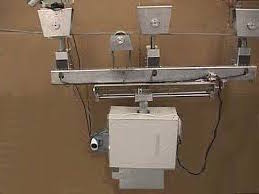
\includegraphics[width=0.5\textwidth]{./roboventrella}
	%\fdireta{ventrella2003robo}			 											 
\end{figure}													 
%----------------------------------------------------------

O conceito de um robô móvel para instalação e remoção autônoma de esferas de sinalização aéreas em linhas de transmissão de energia (Firugar \ref{img:campos}) é apresentado por Campos et al. \cite{campos2002mobile}. Segundo os autores, um computador de bordo é responsável pelo controle através dos dados obtidos pelos sensores e dos comandos enviados por um operador de solo. Os comandos do operador são transmitidos por ondas de rádio, o que permite que o sistema seja remotamente operado a uma distância de até 2 km. O equipamento foi testado em campo em uma situação real e mostrou-se eficiente e robusto. De acordo com Gonçalves e Carvalho \cite{gonccalves2013review}, apesar do mecanismo proposto por Campos et al. \cite{campos2002mobile} não superar obstáculos nem navegar em linhas entre duas torres, é simples e funcional.

%---------------picture------------------------------------
\begin{figure} [h!]	
	\caption{Teste em campo realizado com o robô para instalação e remoção de esferas de sinalização aérea.}
	\label{img:campos}											 
	\centering													 
	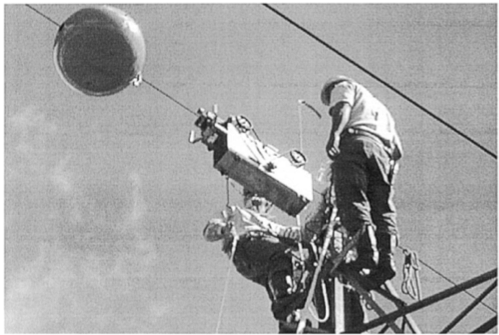
\includegraphics[width=0.6\textwidth]{./campos}
	%\fdireta{campos2002mobile}			 											 
\end{figure}													 
%----------------------------------------------------------

Apoiado pelo financiamento do Plano Nacional Chinês 863, Zhou et al. \cite{zhou2005control} propuseram um robô (Figura \ref{img:zhou}) capaz de ultrapassar qualquer tipo de obstáculo (até torres) ao trafegar ao longo de uma linha de transmissão de até 110 kV. O robô conta com uma câmera; as imagens de inspeção, por sua vez, são enviadas para uma estação de trabalho do solo através de um sistema de comunicação sem fio.  

%---------------picture------------------------------------
\begin{figure} [h!]	
	\caption{Configuração do robô de inspeção.}
	\label{img:zhou}											 
	\centering													 
	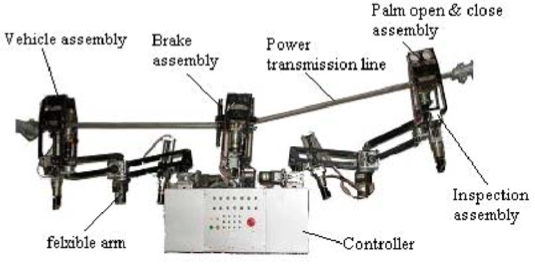
\includegraphics[width=0.6\textwidth]{./zhou}
	%\fdireta{zhou2005control}			 											 
\end{figure}													 
%----------------------------------------------------------

De acordo com a Figura \ref{img:zhou}; a estrutura mecânica do robô desenvolvido por Zhou et al. \cite{zhou2005control} é composta por cinco grandes partes: mecanismo de movimentação (vehicle driving mechanism); sistema de parada (brake system assembly); braços flexíveis (flexible arms); garras (palm gripper); fonte de alimentação e sistema de controle (power supply and controller). Para assegurar a flexibilidade requerida o robô (que pesa cerca de 45 kg e tem 1,2 m de comprimento) tem 16 eixos de movimentação, podendo vencer inclinações de até 60$^{\circ}$. 

Como parte do programa de pesquisa Hydro-Québec Montambault e Pouliot \cite{montambault2007design} encarregaram-se do desenvolvimento de uma tecnologia para inspeção e manutenção de linhas de transmissão de 735 kV, denominada LineScout (Figura \ref{fig:linescout}). Segundo por Montambault e Pouliot \cite{montambault2007design}, o protótipo deste robô móvel tele operado (pesando 100 kg) foi testado e validado em muitas configurações de linhas e de sequências de obstáculos, sob condições de campo.

%------ picture with two parts -------------
\begin{figure}[h!]
		\caption{Robô LineScout.}
%------ picture part a ---------------------
		\begin{subfigure}[b]{0.5\textwidth}
		  	\centering
		  	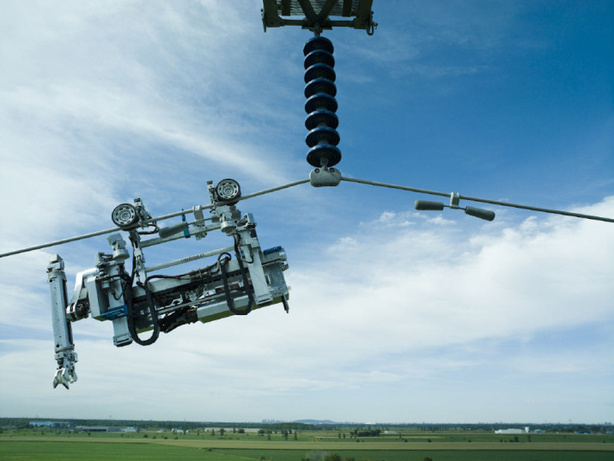
\includegraphics[width=0.9 \textwidth]{./linescout1} 
		  	\caption{robô em operação}
		  	\label{fig:linescout1}
		\end{subfigure} 
%------ picture part a ---------------------
		\begin{subfigure}[b]{0.5\textwidth}
		  	\centering
		  	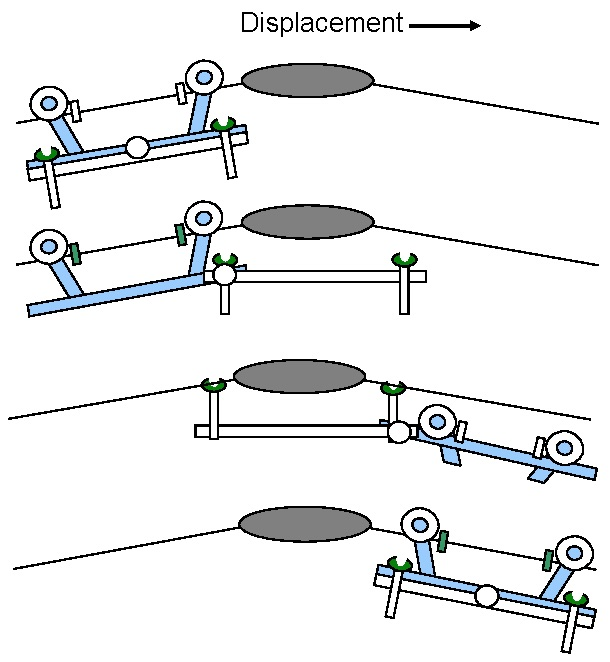
\includegraphics[width=0.6 \textwidth]{./linescout2} 
		  	\caption{esquema de movimentos para ultrapassagem de obstáculos.}
		  	\label{fig:linescout2}
		\end{subfigure} 
%----- info - central picture --------------
	  %\caption{Robô LineScout.} 
	  %\fdireta{montambault2007design} 
	  \label{fig:linescout}
\end{figure}
%-------------------------------------------

O LineScout, como mostrado na Figura \ref{fig:linescout}, utiliza o cabo condutor como suporte; o uso de rodas para movimentação não só possibilita a locomoção rápida e eficiente ao longo da linha, como também permite passar por cima de alguns obstáculos. Para ultrapassar outros tipos de obstáculos é empregada a sequência de movimentos esquematizados na Figura \ref{fig:linescout2}.
Em 2008 Katrasnik, Pernus e Likar \cite{katrasnik2010climbing} propuseram um conceito híbrido para inspeção de linhas de transmissão; o qual combina o uso de um veículo aéreo não tripulado (VANT) e um robô móvel (Figura \ref{img:katrasnik}). Em seus estudos conceituais os autores comparam os três tipos de sistemas para inspeção: os robôs móveis, os por veículos aéreos e os híbridos; concluindo que, apesar da baixa qualidade de inspeção e autonomia, o sistema proposto tem como vantagem a universalidade e a facilidade de projeto.  Katrasnik, Pernus e Likar \cite{katrasnik2010climbing} acreditam ainda que a solução híbrida provavelmente não terá a autonomia de superação de obstáculos possíveis aos robôs móveis tendo, porém, um provável custo menor de desenvolvimento.  

%---------------picture------------------------------------
\begin{figure}[h!]	
	\caption{Robô híbrido e seus componentes.}
	\label{img:katrasnik}											 
	\centering													 
	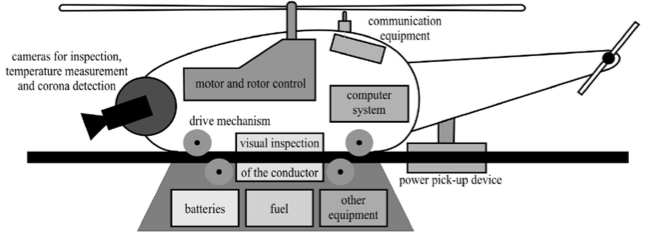
\includegraphics[width=0.8\textwidth]{./katrasnik}
	%\fdireta{katrasnik2010climbing}			 											 
\end{figure}													 
%----------------------------------------------------------

Os primeiros estágios de desenvolvimento do Expliner (Figura \ref{img:expliner1}) são apresentados no artigo de Debenest et al. \cite{debenest2008expliner}. Este robô tele operado foi projetado para realização de manutenção preventiva de linhas de transmissão de alta-voltagem e conta com dois pontos de apoio e um contrapeso.  A movimentação do contrapeso permite que haja o controle da posição do centro de massa e o consequente levantamento em um dos pontos de suporte; este mecanismo possibilita a ultrapassagem de obstáculo (a exemplo do mostrado na Figura \ref{img:expliner2} ).

%------ picture with two parts -------------
\begin{figure}[h!]
		\caption{Robô Expliner.}
%------ picture part a ---------------------
		\begin{subfigure}[b]{0.5\textwidth}
		  	\centering
		  	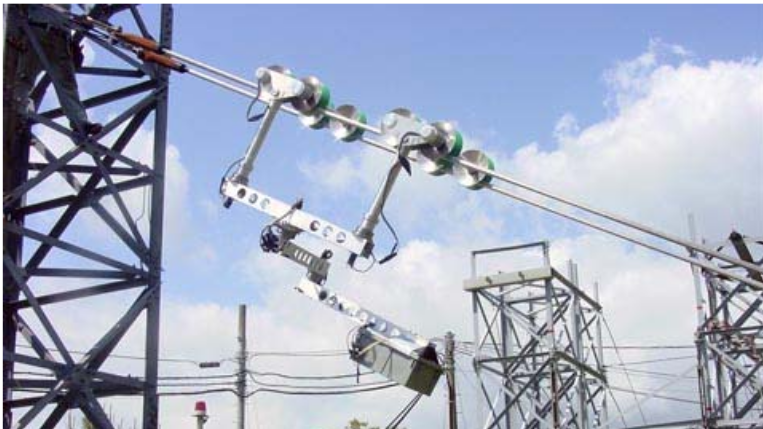
\includegraphics[width=0.9 \textwidth]{./expliner} 
		  	\caption{robô e sua submontagens.}
		  	\label{img:expliner1}
		\end{subfigure}
%------ picture part a ---------------------
		\begin{subfigure}[b]{0.5\textwidth}
		  	\centering
		  	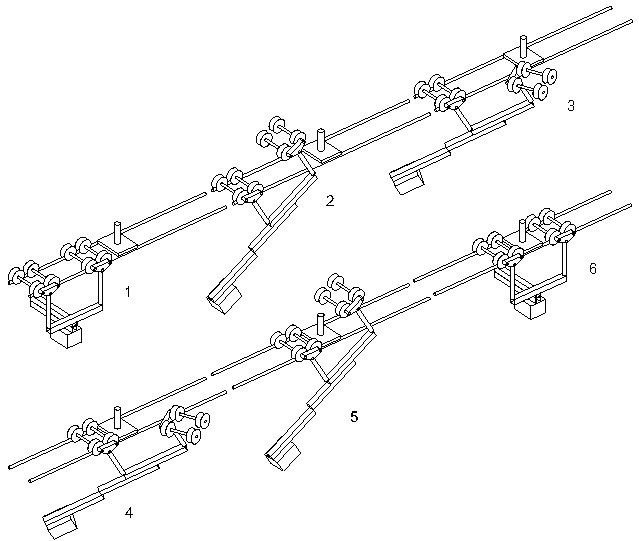
\includegraphics[width=0.6 \textwidth]{./expliner2} 
		  	\caption{esquema de movimentos para ultrapassagem de obstáculos.}
		  	\label{img:expliner2}
		\end{subfigure} 
%----- info - central picture --------------
	  %\caption{Robô Expliner.} 
	  %\fdireta{debenest2008expliner} 
	  \label{img:expliner}
\end{figure}
%-------------------------------------------

De acordo com Debenest et al. \cite{debenest2008expliner}, o Expliner pode ser semi-controlado através de um sistema de comunicação sem fio, ou seja, o usuário está sempre encarregado da sua operação não precisando, porém, controlar todos os detalhes, mas sim autorizar a realização de tarefas pré-programada; as sequências de movimento ficam gravadas na sua memória. Por pesar 84 kg, um cabo de acesso deve ser usado para colocar o robô na linha de transmissão.  De acordo com os autores, os testes realizados mostram que o Expliner pode mover-se até m/min e superar inclinações de até 30 graus. 

Já a proposta de Rangel, Kienitz e Brandão \cite{rangel2009sistema} é o desenvolvimento de uma plataforma de monitoramento aéreo a ser utilizado para inspecionar linhas de alta voltagem. Para tal, a integridade da linha é verificada com o auxílio de um VANT (Figura \ref{img:rangel2}), onde é instaladas câmeras de vídeo, equipamentos de controle e de telemetria. O VANT é pilotado remotamente por um operador que se encontra na estação de solo (Figura \ref{img:rangel2}). As imagens capturadas e os dados georreferenciados da linha e do terreno são enviados, em tempo real, ao solo para posterior armazenamento e processamento.

%---------------picture------------------------------------
\begin{figure} [h!]	
	\caption{VANTs utilizados como plataforma de testes.}
	\label{img:rangel1}											 
	\centering													 
	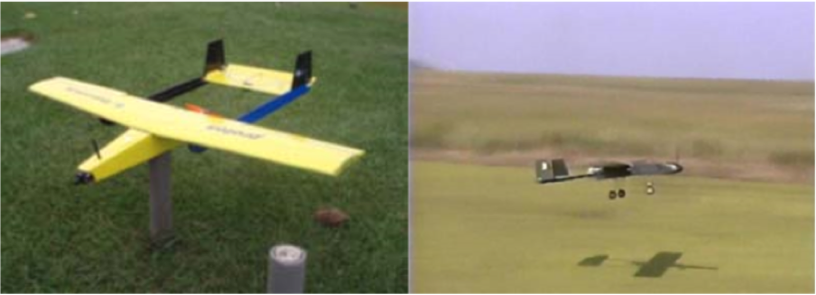
\includegraphics[width=0.6\textwidth]{./rangel}
	%\fdireta{rangel2009sistema}			 											 
\end{figure}													 
%----------------------------------------------------------

%---------------picture------------------------------------
\begin{figure} [h!]	
	\caption{Sistema de monitoramento aéreo para linhas de transmissão de energia.}
	\label{img:rangel2}											 
	\centering													 
	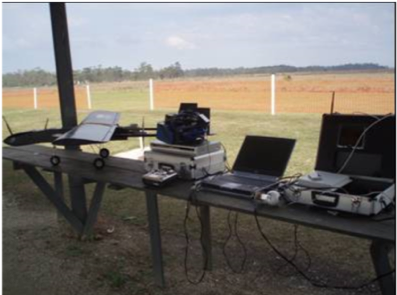
\includegraphics[width=0.6\textwidth]{./rangel2}
	%\fdireta{rangel2009sistema}			 											 
\end{figure}													 
%----------------------------------------------------------

Durante a pesquisa da inspeção utilizando VANTs, foi constatado que estes não substituem com plenitude as aeronaves tripuladas nesta tarefa, uma vez que existem limitações quanto à proximidade dos veículos com a linha de transmissão para que não haja interferência eletromagnética no sistema. Os autores citam ainda, que esta proposta presta-se, fundamentalmente, a identificação e diagnóstico do problema, não sendo possível a realização de manutenção corretiva (como ocorre quando há a inspeção por helicóptero tripulado).  
Li e Ruan \cite{li2010autonomous} em seu trabalho descrevem o desenvolvimento de um robô móvel para inspeção de linhas de transmissão de 500 kV capaz de superar alguns obstáculos como contrapesos, torre de ancoragem, e torres de torção (Figura \ref{img:li} ). O robô projetado conta com treze motores e tem sua mobilização, inspirada no comportamento dos macacos. Estruturado em um mecanismo formado por engrenagens sem-fim, rodas, garras, parafusos e porcas ele tem capacidade para escalar linhas com no máximo 60 graus. O protótipo deste robô, (com 30 kg e tem 1,2 m de comprimento e 0,8 m de altura) ainda está em fase de desenvolvimento e carece de uma maior robustez para a efetiva realização de algumas inspeções necessárias para uma boa manutenção preventiva das linhas de transmissão.

%---------------picture------------------------------------
\begin{figure} [h!]	
	\caption{Teste do robô de inspeção.}
	\label{img:li}											 
	\centering													 
	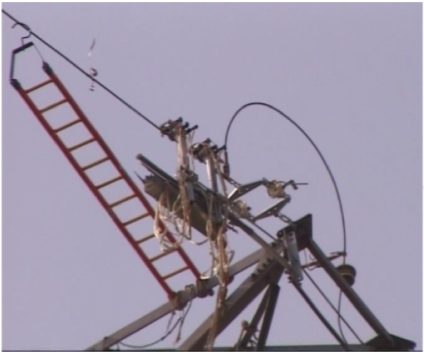
\includegraphics[width=0.6\textwidth]{./li}
	%\fdireta{li2010autonomous}			 											 
\end{figure}													 
%----------------------------------------------------------

O robô proposto por Wang et al. \cite{wang2010design} apresentam um mecanismo diferenciado para a realização da inspeção de linhas de transmissão. Como pode ser observado na Figura \ref{img:wang}, este robô móvel conta com uma estrutura bípede e os seus dois pés podem ser presos à linha de transmissão; os seus ciclos de movimento sob a linha são compostos por fases onde há um único apoio e outras fases onde há dois apoios. Cada perna tem uma junta prismática que permite que o seu tamanho seja ajustado fazendo com que o seu centróide sempre coincida com o eixo da articulação central (hip joint), reduzindo o consumo de energia e mantendo a sua estabilidade na quando o robô está mono apoiado. 

%---------------picture------------------------------------
\begin{figure} [h!]	
	\caption{Modelo 3D do robô bípede para inspeção de linhas de transmissão.}
	\label{img:wang}											 
	\centering													 
	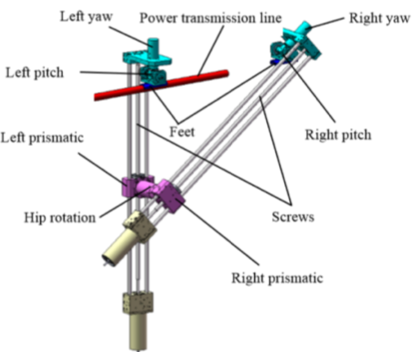
\includegraphics[width=0.6\textwidth]{./wang}
	%\fdireta{wang2010design}			 											 
\end{figure}													 
%----------------------------------------------------------

O protótipo do robô apresentado por Wang et al. \cite{wang2010design} possui 800 mm de altura e 100 mm de largura, quando todas as juntas estão na posição zero; o maior obstáculo que pode transpor tem 300 mm de comprimento. Os autores concluem que os próximos trabalhos a serem realizados com este protótipo devem focar na inclusão de sensor de detecção de linha, controle on-board e testes em ambientes reais de linha de transmissão e obstáculos.  
O “Cable Crawler” é tratado por Buehringer et. al \cite{buhringer2010cable}, um robô tele operado para inspeção de linha de transmissão de alta voltagem que trafega ao longo do cabo terra. Este robô, que pesa 53 kg, conta com um mecanismo que permite com que ele transponha desde pequenos obstáculos até as torres (como mostrado na Figura 18). 

%---------------picture------------------------------------
\begin{figure} [h!]	
	\caption{Demonstração da sequência de movimentos do Cable Crawler ultrapassando uma torre.}
	\label{img:buehringer}											 
	\centering													 
	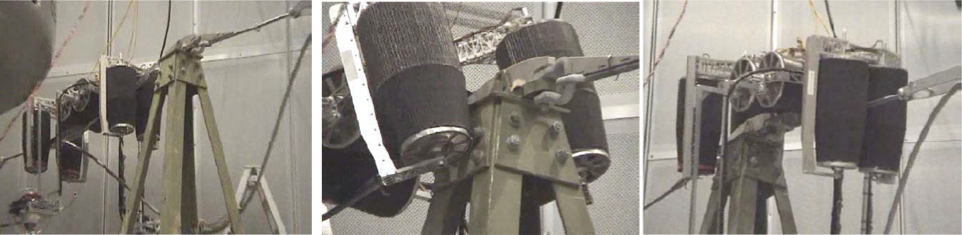
\includegraphics[width=0.6\textwidth]{./buehringer}
	%\fdireta{buhringer2010cable}			 											 
\end{figure}													 
%----------------------------------------------------------

Gonçalves e Carvalho em seus trabalhos \cite{goncalves2010graphical} \cite{gonccalves2013review}  apresentam os resultados dos estudos desenvolvidos a cerca de um robô móvel suspenso por fio projetado para manutenção e inspeção de linhas de energia e/ou telecomunicação. Segundo Gonçalves \cite{gonccalves2006kinematics} este robô, de fácil controle, tem a capacidade de transpor alguns obstáculos, como por exemplo grampos e esferas de sinalização, independentemente de sua posição; uma vez que é dotado de quatro pernas de comprimentos variáveis.

%---------------picture------------------------------------
\begin{figure} [h!]	
	\caption{Configuração geral do robô suspenso por fio com pernas iguais.}
	\label{img:goncalves}											 
	\centering													 
	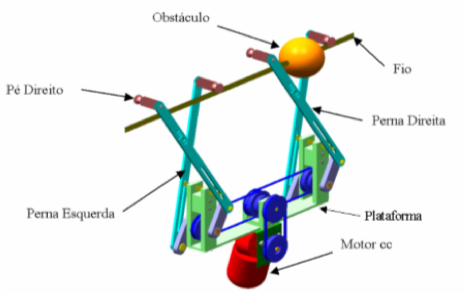
\includegraphics[width=0.6\textwidth]{./goncalves}
	%\fdireta{gonccalves2006kinematics}			 											 
\end{figure}													 
%----------------------------------------------------------

A Figura \ref{img:goncalves} ilustra a configuração geral do robô proposto por Gonçalves e Carvalho \cite{gonccalves2006kinematics} \cite{goncalves2010graphical}. Um dos princípios do seu desenvolvimento é a  facilidade de controle, para tal, a movimentação das quatro pernas é sincronizada por um conjunto de polias e correias acionado por um único motor. 
O Instituto Coreano de Pesquisa em Energia Elétrica propõe, através do trabalho de Lee, Jung e Cho \cite{lee2011development}, um robô para inspeção de luvas de emenda de linhas de transmissão pela medição do campo magnético. O seu programa de interface com o usuário (remoto) mostra a condição da ferramenta, permitindo com que o operador comande os movimentos do robô; além de calcular e apresentar o grau de excentricidade da luva.  

%---------------picture------------------------------------
\begin{figure} [h!]	
	\caption{Equipamento para inspeção de luvas de emendas de linhas de transmissão.}
	\label{img:lee}											 
	\centering													 
	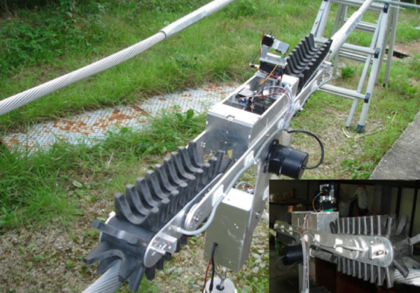
\includegraphics[width=0.6\textwidth]{./lee}
	%\fdireta{lee2011development}			 											 
\end{figure}													 
%----------------------------------------------------------

Como pode ser visto na Figura \ref{img:lee}, a estrutura do robô para inspeção de luvas de emendas é formada de duas partes: uma responsável pelo movimento e outra pela inspeção. De acordo com Gonçalves e Carvalho \cite{gonccalves2013review}, seu deslocamento assemelha-se a uma lagarta, onde há aderência e locomoção ao longo do cabe através de um sistema de sulcos e ranhuras que permite que o robô supere elevações e depressões sem cair.

Phillips et al. \cite{phillips2012autonomous} apresentaram em seu trabalho o robô que autonomamente inspeciona linhas de transmissão de alta voltagem desenvolvido pelo Electric Power Research Institute (EPRI); denominado Ti. No campo, este robô é instalado permanentemente à linha de transmissão e é capaz de transpor os obstáculos através de sistemas de by-pass, também permanentes. O Ti dispõe de câmeras de alta definição, câmaras espectro de infravermelho, detectores de interferência eletromagnética e diversos sensores de radiofrequência; os autores acreditam que, desta maneira, o sistema será capaz de fornecer informações completas, precisas e úteis para otimizar a manutenção de linha e melhorar a confiabilidade da transmissão. 

%---------------picture------------------------------------
\begin{figure} [h!]	
	\caption{Robô Ti em teste.}
	\label{img:phillip}											 
	\centering													 
	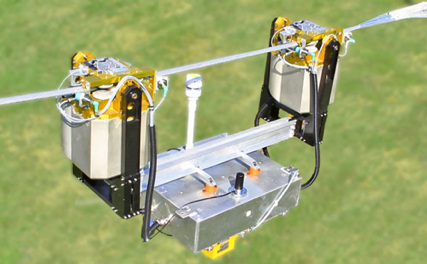
\includegraphics[width=0.6\textwidth]{./phillip}
	%\fdireta{phillips2012autonomous}			 											 
\end{figure}													 
%----------------------------------------------------------

Baseado na proposta de Katrasnik, Pernus e Likar \cite{katrasnik2010climbing}, Gonçalves e Carvalho \cite{gonccalves2013review} expõem seus estudos a cerca da ideia de um robô modular (Figura \ref{img:goncalvesecarvalho}). Nesta solução cada módulo possuirá sua própria movimentação, função e sistema de energia, podendo transitar ao longo do cabo de alta voltagem ou do de terra. O primeiro módulo carregará um UAV, veículo que será responsável pelo carregamento de todos os módulos no momento da ultrapassagem de obstáculos, podendo ser tele operado. Existirá ainda, o módulo incumbido da troca de baterias dos demais. 

%---------------picture------------------------------------
\begin{figure} [h!]	
	\caption{Robô modular.}
	\label{img:goncalvesecarvalho}											 
	\centering													 
	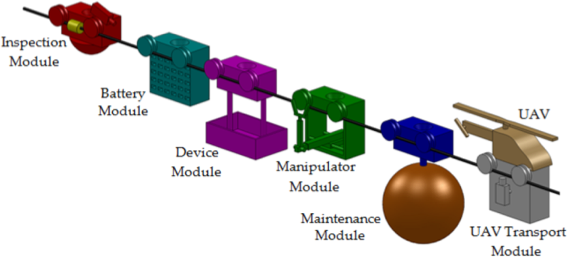
\includegraphics[width=0.6\textwidth]{./goncalvesecarvalho}
	%\fdireta{gonccalves2013review}			 											 
\end{figure}													 
%----------------------------------------------------------

Gonçalves e Carvalho \cite{gonccalves2013review} acreditam que, uma vez que cada módulo possuirá uma finalidade específica, haverá a otimização do seu peso total (dependendo da atividade) reduzindo o consumo de energia. Os autores afirmam, ainda, diante da individualidade dos módulos, que o robô poderá ser projetado para diversas tarefas (inspeção, manutenção, instalação, limpeza, captura de imagens, etc.) sem necessariamente ser pesado e grande (como seria um robô monobloco multitarefa). 

%------

Destacaremos no presente trabalho o robô autônomo apresentado por Lima II et al. \cite{iirobo} e Mourão et al. \cite{mourao2015robolinhas} denominado PIRO (Powerlines Inspection Robot) ou D311, fruto da parceria entre CEMIG, SENAI-CIMATEC/BIR (Brazilian Institute of Robotics) e Universidade Federal de Minas Gerais (no âmbito do Programa de Pesquisa e Desenvolvimento Tecnológico do Setor de Energia Elétrica regulado pela ANEEL). 

%---------------picture------------------------------------
\begin{figure} [h!]	
	\caption{Esboço inicial do PIRO.}
	\label{img:piro}											 
	\centering													 
	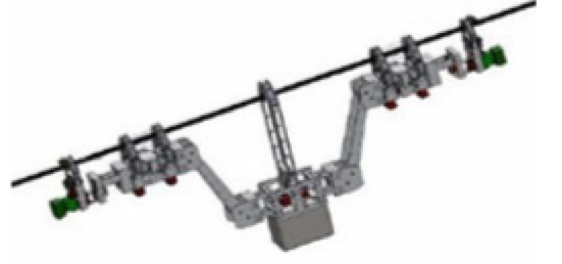
\includegraphics[width=0.6\textwidth]{./piro}
	%\fdireta{iirobo}			 											 
\end{figure}													 
%----------------------------------------------------------

De acordo com os autores, o projeto do PIRO tem como objetivo ser uma proposta inovadora diante dos resultados encontrados anteriormente por outros pesquisadores; sendo autônomo para a realização de inspeção visual e térmica de cabos de transmissão de linhas energizados e transposição automatizada de obstáculos. Para tanto se considerou como pré-requisitos que o robô deve:

\begin{itemize}
	\item Trabalhar em uma faixa de tensão entre 124,2 kV e 151,8 kV com corrente trifásica de 500 A.
	\item Ser autônomo, dependendo de operadores apenas para sua instalação e remoção no trecho a ser inspecionado ou por eventuais paradas emergenciais.
	\item Operar em um cabo condutor LINNET, com diâmetro de 18,3 mm.
	\item Ter massa menor ou igual a 14 kg, permitindo a instalação em campo com a utilização de hastes por apenas dois operadores. 
	\item Ser provido de blindagem elétrica e magnética de forma a assegurar seu funcionamento na linha de transmissão, ou seja, que não haja danos nos seus componentes devido aos campos eletromagnéticos intensos.
	\item Ser capaz de transportar sensores e equipamentos para inspeção visual e térmica, diagnosticando possíveis falhas no sistema que podem interferir no fornecimento de energia elétrica.
\end{itemize}

Lima II et al. \cite{iirobo} e Mourão et al. \cite{mourao2015robolinhas} afirmam que o mecanismo do D311 para superação de obstáculo foi inspirado no movimento na lagarta Caterpillar (Figura \ref{img:dubois} ). De acordo com a Figura \ref{img:piro2} , optou-se, ainda, por uma estrutura mecânica modular composta por: Braços, os quais unem a unidade de tração e de apoio. O módulo de tração, responsável pela força motora. Unidade de apoio, a qual atua como ponto de referência do equipamento e funciona como mais um ponto de suporte durante a rotina de ultrapassagem de obstáculos. 

%---------------picture------------------------------------
\begin{figure} [h!]	
	\caption{Movimento da lagarta Caterpillar.}
	\label{img:dubois}											 
	\centering													 
	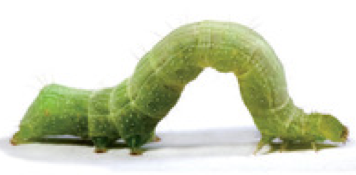
\includegraphics[width=0.6\textwidth]{./dubois}
	%\fdireta{dubois2010complex}			 											 
\end{figure}													 
%----------------------------------------------------------

%---------------picture------------------------------------
\begin{figure} [h!]	
	\caption{Configuração básica da segunda versão do robô PIRO.}
	\label{img:piro2}											 
	\centering													 
	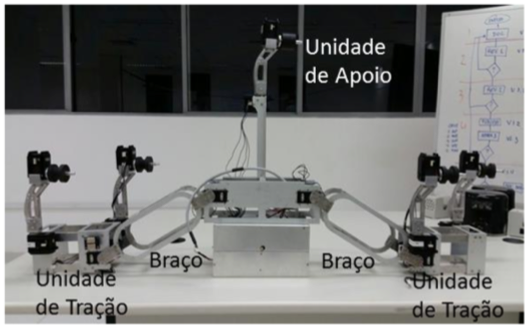
\includegraphics[width=0.6\textwidth]{./piro2}
	%\fdireta{mourao2015robolinhas}			 											 
\end{figure}													 
%----------------------------------------------------------

O PIRO conta com uma estrutura simétrica, que o permite deslocar em ambos os sentidos sem que haja a necessidade de desacoplamento do robô; além de quatro articulações, que provém o número de GDLs necessários seu funcionamento adequado. Sua estrutura é fabricada através de perfis metalon de liga alumínio 2024-T6, o que garantiu redução de tempo de produção, custo e, principalmente, peso. Os autores acreditam que, uma vez que o braço do PIRO tem apenas 153 g e toda a estrutura mecânica tem 1,8 kg; alcançou-se uma inovação ímpar ao estado-da-arte, a massa total da estrutura final do robô é 8,92 kg.
Segundo Mourão et al. \cite{mourao2015robolinhas}, durante os testes realizados em laboratório foi constatado: que a morfologia do robô permite que a transposição de obstáculo; que o sistema de acionamento responde de forma precisa aos comandos de deslocamento, velocidade e aceleração além da rapidez e eficácia do sistema de sensoriamento e visualização. Já os testes executado em linha viva de 138 kV, para verificação quanto à susceptibilidade às interferências eletromagnéticas, sendo que os resultados mostram-se satisfatórios. 
O artigo Lima II et al. \cite{iirobo} traz, ainda, um estudo comparativo entre o D311 e outros robôs para inspeção de linhas de alta tensão. Em relação ao LineScout, apresentado por Montambault e Pouliot \cite{montambault2007design} , o PIRO tem a vantagem de ser autônomo (e não tele operado), ou seja, não depende da habilidade do operador; além de ter massa sete vezes menor, permitindo o seu acoplamento manual. A utilização dos VANTs, por sua vez, apesar da sua maior velocidade de inspeção, em comparação com o D311 apresenta as desvantagens da necessidade de extensa área para pouso e decolagem, menor exatidão na localização dos defeitos, grande influência de perturbações externas e taxas de amostragem insuficientes para elevadas velocidades de varredura.
....


%--------- NEW SECTION ----------------------
\section{Descrição do sistema}
\label{sec:desc}

As concessionárias de energia elétrica e diversas instituições de pesquisa, nos últimos anos vêm trabalhando na busca de uma solução para a inspeção de linhas de transmissão de alta tensão. A abrangência de suas pesquisas perfazem em grande parte no desenvolvimento de robôs para realizar a inspeção. 
Esta tese tomou como base o sistema mecânico desenvolvido no projeto do primeiro robô de inspeção de linha de transmissão brasileiro de baixo peso, apresentado no VII Congresso de Inovação Tecnológica em Energia Elétrica \cite{mourao2015robolinhas}.
A escolha no uso desta solução mecânica originou-se dos resultados alcançados por este projeto diante dos desafios de uma inspeção de linhas de transmissão. Denominado projeto D311 e sob o código Aneel PD-4950-0311/2011, teve como objetivo desenvolver um robô autônomo para executar a inspeção visual e térmica de linhas de transmissão de alta tensão (138kV), realizando automaticamente a transposição de obstáculos presentes na linha de transmissão.
Apesar de alcançar os objetivos inicialmente traçados, o sistema de navegação do robô não era autônomo, seu deslocamento e transposição era baseado em reconhecimentos de padrões e todos os algoritmos pré-estabelecidos eram acionados quando do reconhecimento do padrão.

Diante da ideia estabelecida, esta tese promoveu algumas modificações nas estruturas mecânicas para simplificar as modelagens necessárias para a simulação, logo em termos estruturais e dimensionais a estrutura mecânica proposta apresenta modificações consideráveis em relação ao robô do Projeto D311. Para dar suporte a compreensão deste modelo proposto, os desenhos mecânicos desenvolvidos são apresentados no Apêndice \ref{appendix:meca}. Uma das principais diferenças entre a proposta do robô desta tese e do PIRO apresentado por \citeonline{mourao2015robolinhas}, está no fato deste realizar a detecção e classificação de objetos de forma autônoma, além de desempenhar autonomamente as funções de translação e transposição. Outro ponto a ser considerado é a sua flexibilidade em transpor obstáculos, o robô em questão terá uma capacidade de desempenho maior do que o apresentado por \cite{mourao2015robolinhas}; quanto a sua montagem, o robô apresenta simplicidades na fabricação das peças além de possibilidade um número maior de graus de liberdade necessárias para os movimentos. A proposta para o robô é apresentada na figura \ref{img:elir}.

%---------------picture------------------------------------
\begin{figure} [h!]	
	\caption{Protótipo do robô ELIR.}
	\label{img:elir}											 
	\centering													 
	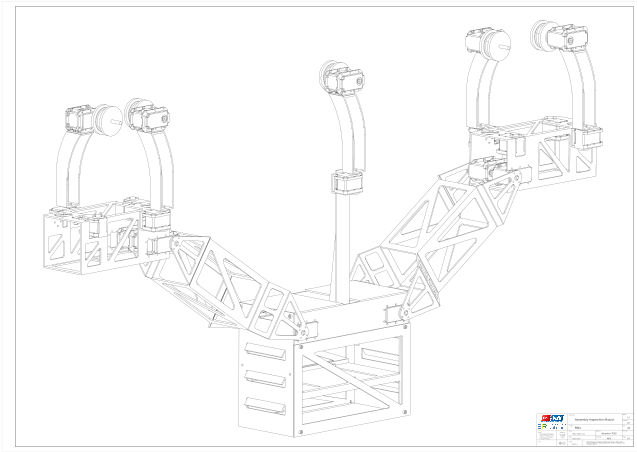
\includegraphics[width=0.7\textwidth]{./elir}
	%\fautor			 											 
\end{figure}													 
%----------------------------------------------------------

Este protótipo será referenciado como robô ELIR, o qual recebe este nome devido a sua representação de Robô de Inspeção Elétrica em inglês, ou seja Electrical Inspection Robot. O ELIR é composto por duas unidades de tração, dois "braços", e uma unidade central. A unidade de tração é composta por um par de garras, com um servomotor e uma roda em cada uma, além disso a estrutura principal da unidade é composta por mais dois servomotores com o objetivo de deslocar as garras da unidade. Os braços são compostos por uma estrutura metálica em alumínio, na extremidade de cada um deles há uma junta de movimentação composta por dois servomotores. A unidade central é onde o processamento do robô se encontra, a unidade também agrega o subsistema de potência do robô.

A proposta do sistema mecânico aqui apresentada foi estudada e simulada por \citeonline{sartori2018}, que diante do dimensional sugerido pela Figura \ref{img:vistaselir} realizou uma análise geométrica do referido sistema robótico ELIR, chegando a conclusão de que não havia interferência mecânica entre a estrutura do robô e os obstáculos durante o processo de movimentação ou de transposição.

%---------------picture------------------------------------
\begin{figure} [h!]	
	\caption{Vista frontal e laterial do robô ELIR.}
	\label{img:vistaselir}											 
	\centering													 
	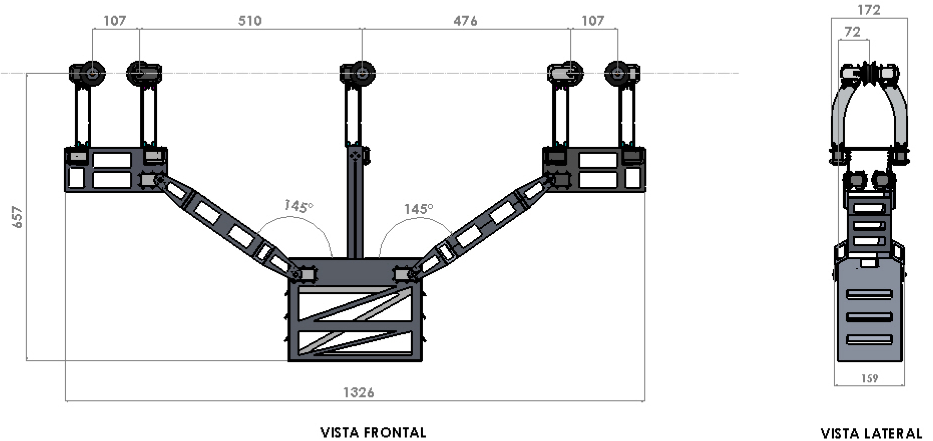
\includegraphics[width=0.7\textwidth]{./vistaselir}
	%\fautor			 											 
\end{figure}													 
%----------------------------------------------------------

 De forma resumida, os dimensionais do sistema robótico é apresentado na Figura \ref{img:vistaselir} e tomando como referência a Figura \ref{img:esquemaelir} juntamente com seus parâmetros e matrizes de transformação, chega-se a conclusão que há uma simetria na geometria do robô ELIR, bastando dessa forma permutar entre a base e o efetuador, ou seja as matrizes da cinemática direta são válidas para as duas extremidades.

%---------------picture------------------------------------
\begin{figure} [h!]	
	\caption{Esquema do ELIR  com os sistemas de coordenadas das suas articulações, para a verificação do deslocamento das roldanas das unidades de tração.}
	\label{img:esquemaelir}											 
	\centering													 
	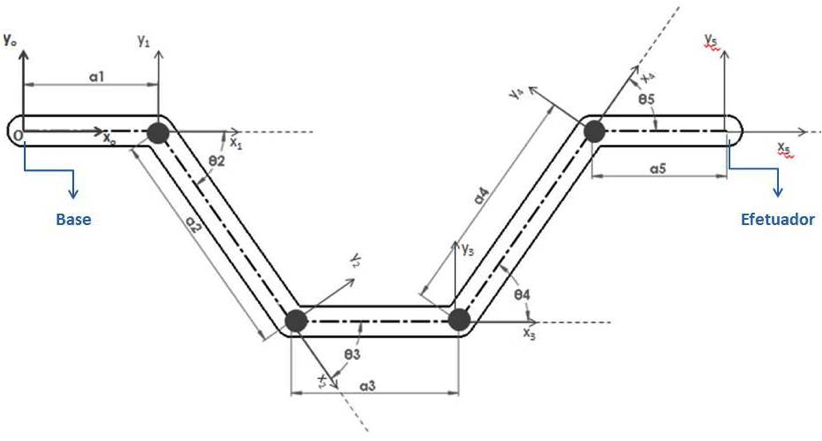
\includegraphics[width=0.7\textwidth]{./esquemaelir}
	%\fautor			 											 
\end{figure}													 
%----------------------------------------------------------

Consequentemente, tomando o sistema e dividindo-o em cinco partes, as matrizes homogêneas do robô são estabelecidas, levando em consideração os parâmetros de Denavit-Hartenberg apresentado na Tabela \ref{tab:parametrodhelir} para o robô ELIR, no qual chega-se aos valores dimensionais dos ângulos de cada junta (Figura \ref{img:esquemaelirdim}) obtidos na análise cinemática.

%----------------table-------------------------------------
\begin{table}[htb!]
	\caption{Parâmetros de DH do ELIR , para a verificação do deslocamento das roldanas das unidades de tração}
	\label{tab:parametrodhelir}
	\centering
	%\begin{tabularx}{\textwidth}{X|l|r|r|r} \hline
	\begin{tabular}{c|c|c|c|c}
		Junta    & ai & di & $\alpha i$ & $\theta  i$ \\ \hline
		1        & a1 & 0  & 0        & $\theta 1$  \\
		2        & a2 & 0  & 0        & $\theta 2$  \\
		3        & a3 & 0  & 0        & $\theta 3$  \\
		4        & a4 & 0  & 0        & $\theta 4$  \\
		5        & a5 & 0  & 0        & $\theta 5$  \\ \hline
	\end{tabular}
	%\fdireta{sartori2018}
\end{table}
%----------------------------------------------------------

%---------------picture------------------------------------
\begin{figure} [h!]	
	\caption{Configuração de juntas, ângulos e links para validação da matriz homogênea obtida na ánalise cinemática.}
	\label{img:esquemaelirdim}											 
	\centering													 
	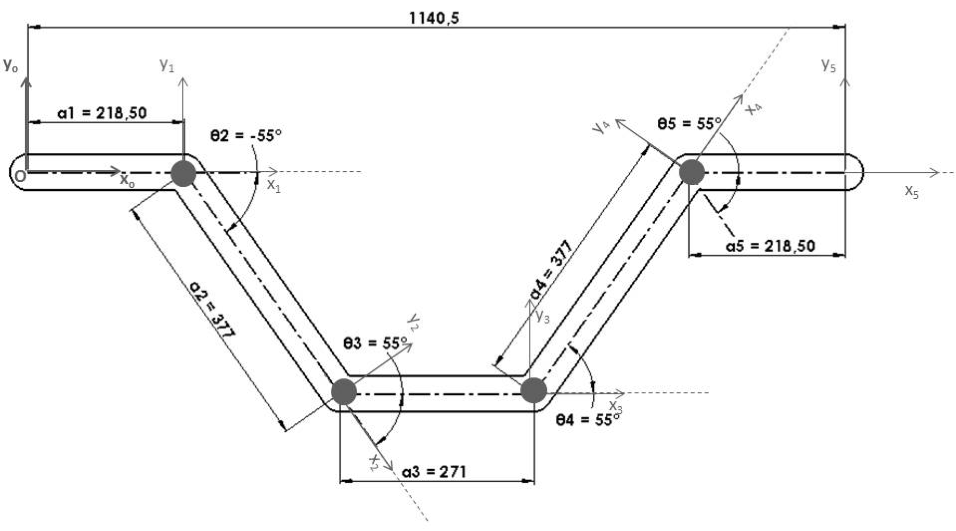
\includegraphics[width=0.9\textwidth]{./esquemaelirdim}
	%\fautor			 											 
\end{figure}													 
%----------------------------------------------------------

A matriz homogênea de cada parte é dada pela Equação \ref{eq:mathomog}. 

%---------------equation-----------------------------------
\begin{equation}
\label{eq:mathomog}
	{A}_{n-1}^{n}=\left (
	\begin{matrix}
 		\cos{\theta}_{n} & -\sin{\theta}_{n} & 0 & {a}_{n}\cos{\theta}_{n} \\ 
 		\sin{\theta}_{n} & \cos{\theta}_{n} & 0 & {a}_{n}\sin{\theta}_{n} \\ 
		0 & 0 & 1 & 0 \\
		0 & 0 & 0 & 1
	\end{matrix}
\right )
\end{equation}
%----------------------------------------------------------

Logo levando-se em consideração que o efetuador do robô esteja numa extremidade, tem-se a matriz transformação homogênea da base definida pela expressão \ref{eq:mathomogbase}.

%4.2
%---------------equation-----------------------------------
\begin{equation}
\label{eq:mathomogbase}
	{A}_{0}^{5}={A}_{0}^{1}\cdot {A}_{1}^{2}\cdot{A}_{2}^{3}\cdot {A}_{3}^{4}\cdot{A}_{4}^{5}=\left (
	\begin{matrix}
 		{r}_{1,1} & {r}_{1,2} & {r}_{1,3} & {x}_{0}^{5} \\ 
 		{r}_{2,1} & {r}_{2,2} & {r}_{2,3} & {y}_{0}^{5} \\ 
 		{r}_{3,1} & {r}_{3,2} & {r}_{3,3} & {z}_{0}^{5} \\
 		0 & 0 & 0 & 1
	\end{matrix}
\right )		
\end{equation}
%----------------------------------------------------------
 
Os elementos da matriz apresentada pela equação xx, são definidos por \citeonline{sartori2018} e serão tomados como parâmetros para esta pesquisa, diante disso chega-se aos dimenstionais apbraesentados na Figura \ref{img:esquemaelirdim} com seus respectivos valores de ângulos, logo podemos encontrar o resultado numérico para a Equação \ref{eq:mathomognum}.

%4.3
%---------------equation-----------------------------------
\begin{equation}
\label{eq:mathomognum}
	{A}_{0}^{5}=\left (
	\begin{matrix}
 		1 & 0 & 0 & 1140.5 \\ 
 		0 & 1 & 0 & 0 \\ 
 		0 & 0 & 1 & 0 \\
 		0 & 0 & 0 & 1
	\end{matrix}
\right )	
\end{equation}
%----------------------------------------------------------

Com isto, pode-se definir qualquer posição do efetuador no espaço de trabalho considerado, assim como identificar as limitações do robô para os movimentos requeridos. Estas definições serão úteis para a elaboração da simulação pretendida nesta tese.

Vale ressaltar que toda estruturação metálica, com seus dimensionais são apresentados ao final da tese na seção Apêndice, mais especificamente no Apêndice \ref{Append:diagmec}. Um outro ponto importante a se destacar, é que a análise cinemática inversa analisada e simulada por \citeonline{sartori2018} não foi considerada para o desenvolvimento desta tese, em subistituição a modelagem matemática será adotado o software \textit{MoveIt!} para estabelecer os posicionamentos das juntas para a realização de uma determinada estratégia a qual se queira desenvolver.

Baseado no conceito inicial do robô, deve-se projetar também os esquemas elétrico e eletrônico do sistema robótico. De forma abrangente a Figura \ref{img:elirmodesq} apresenta o modelo esquemático adotado neste robô.

%---------------picture------------------------------------
\begin{figure} [h!]	
	\caption{Modelo esquemático do robô ELIR.}
	\label{img:elirmodesq}											 
	\centering													 
	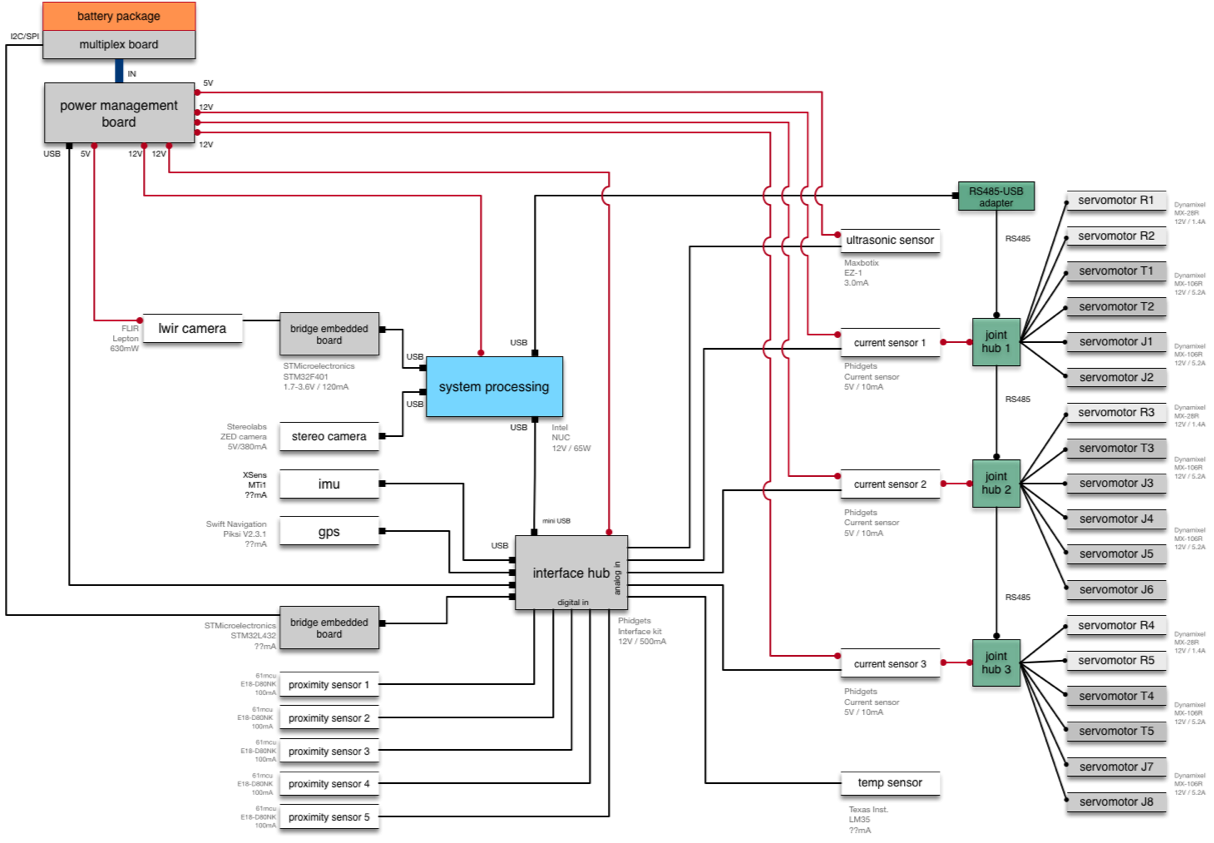
\includegraphics[width=1.0\textwidth]{./modeloesquematico2}
	%\fautor			 											 
\end{figure}													 
%----------------------------------------------------------

Como pode-se observar e de forma abrangente, os principais elementos que compõem o robô são:

\begin{itemize}
	\item 13 servomotores de 8.4Nm
	\item 05 servomotores de 2.5Nm
	\item 01 interface de IO
	\item 01 IMU
	\item 01 GPS
	\item 01 câmera stéreo
	\item 01 câmera LWIR
	\item 05 sensores de proximidade
	\item 01 sensor ultrassônico
	\item 01 sensor de temperatura
	\item 03 sensores de corrente
	\item 01 computador central para processamento das informações
	\item 01 placa de gerenciamento de energia
	\item 01 placa de gerenciamento de baterias
	\item 02 baterias de 12V
\end{itemize}

A Figura \ref{img:elirmodesq} é somente uma representação esquemática para o desenvolvimento da tese, no Apêndice \ref{appendix:elet} é apresentado os diagramas elétricos e eletrônicos para a compreensão total do sistema eletro-eletrônico considerado para este trabalho.

%--------- NEW SUB SECTION ----------------------
%\subsection{Especificação técnica}
%\label{ssec:espt}


%--------- NEW SUB SECTION ----------------------
\subsection{Arquitetura geral do sistema}
\label{ssec:arqg}
Para que o objetivo principal fosse atendido, a arquitetura do sistema foi elaborado compreendendo como um processo constituído de entradas e saídas, conforme representado pela Figura \ref{img:elirarq} . Logo, na arquitetura desenvolvida tem-se uma região sendo considerada como a região onde os sensores são os agentes coletores dos eventos desempenhado pelo robô; concomitantemente as saídas são consideradas como os atuadores que realizam a transposição e a translação do robô, nesta região faz parte também os displays de acesso as informações enviadas pelo robô, assim como a visualização da interface com o robô e o usuário.

%---------------picture------------------------------------
\begin{figure} [h!]	
	\caption{Arquitetura do robô ELIR.}
	\label{img:elirarq}											 
	\centering													 
	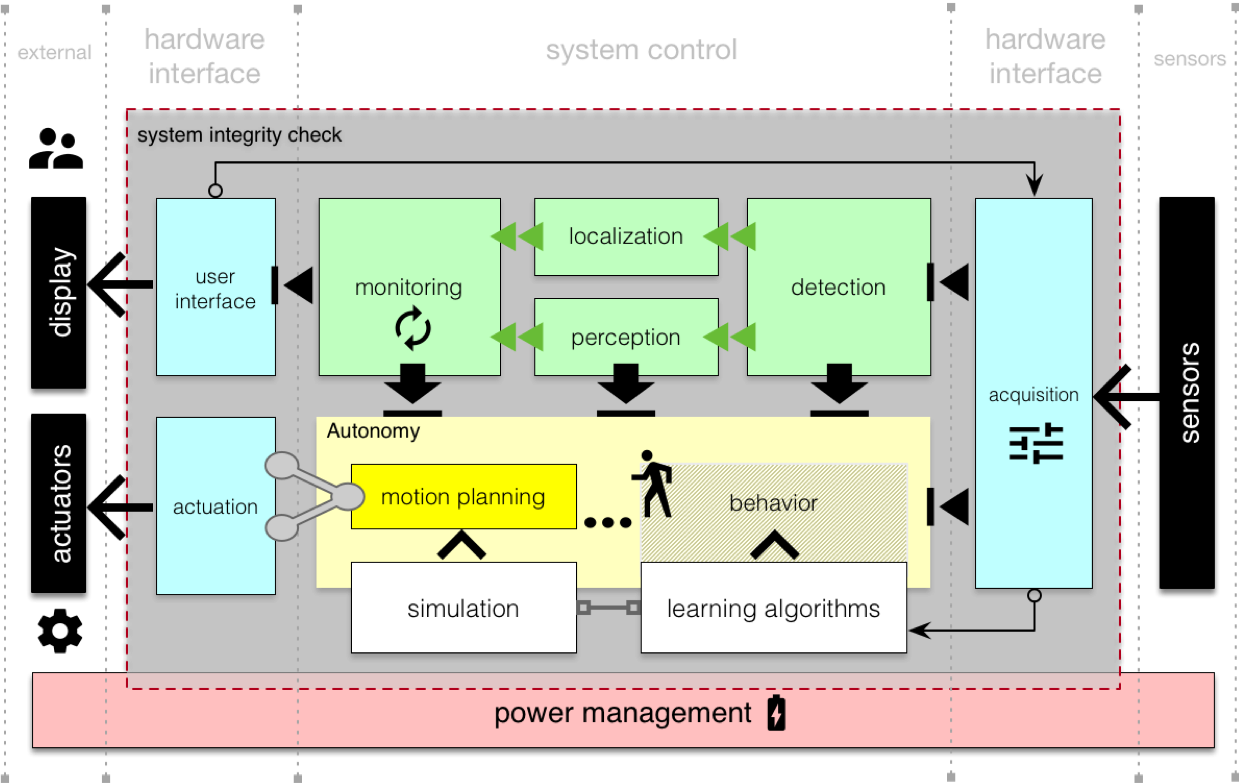
\includegraphics[width=1.0\textwidth]{./arquitetura2}
	%\fautor			 											 
\end{figure}													 
%----------------------------------------------------------

%continuar explicação


A estrutura da arquitetura apresentada basea-se no \textit{framework} ROS, o qual possibilita a integração de todas as funcionalidades necessárias para o desenvolvimento do sistema robótico, trabalhando no conceito de nós, o \textit{framework} facilita a identificação de problemas durante a fase de desenvolvimento e também a modularização dos códigos.

%--------- NEW SUB SUB SECTION ------------------
\subsubsection{Arquitetura do sistema de movimentação}
De forma a garantir uma movimentação efetiva do robô é necessária a integração de diversos ferramentas físicas e de software, como a estrutura de movimentação adequada, sistema ordenamento de missão, controle de potência,demandando assim um \textit{framework} e um sistema operacional.

A inspeção de linha foi denominada missão, para cade vez que o robô começar a realizar a inspeção, será considerado o início de uma nova missão. 

Para garantir a execução correta da missão e ultrapassagem dos obstáculos de forma efetiva, se dividiu o sistema em 4 principais subsistemas, sendo elas : \textit{Motion Planning} , \textit{Actuation},\textit{System Integrity Check} e \textit{Power Management}. A arquitetura geral do sistema de movimentação está mostrada na figura \ref{fig:arq_geral}, ilustrando os subsistemas e suas funcionalidades. 
\begin{figure}[h]
	\centering
	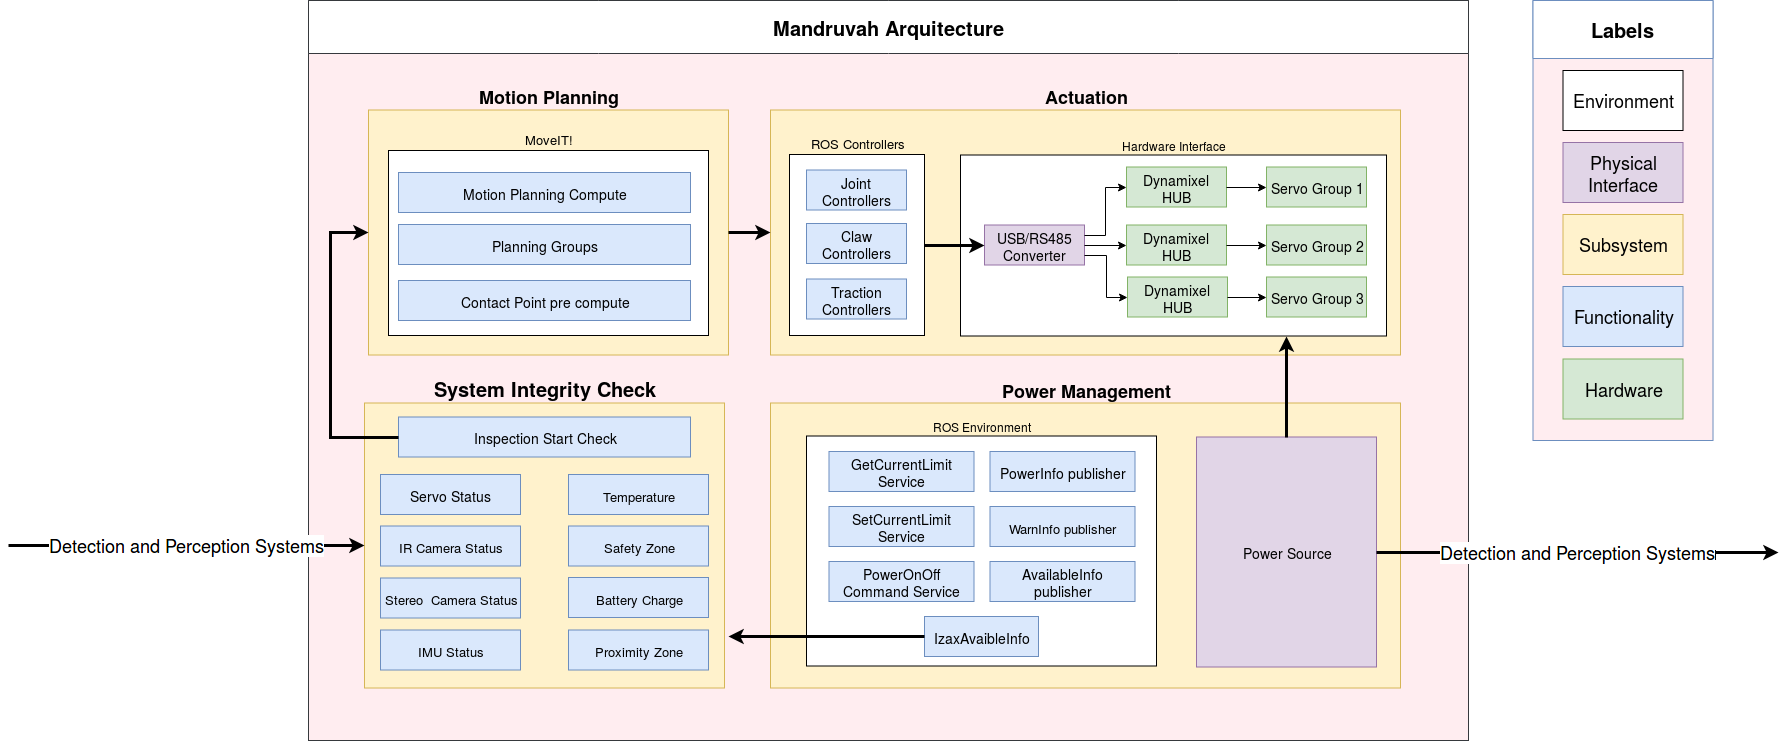
\includegraphics[width=1\textwidth]{Arquitetura.png}
	\caption{Arquitetura Geral do sistema de movimentação}
	\label{fig:arq_geral}
	\source{Própria}
\end{figure} 
A estrutura física do robô foi projetada para que sejam realizados movimentos de translação e transposição de obstáculos presentes na linha de transmissão,consistindo de unidades de tração para a translação na linha e juntas nos braços e garras para a realização da ultrapassagem de obstáculos. O controle da estrutura física do robô está relacionado com a \textit{Actuation}.
A transposição dos obstáculos é um grande desafio para essa aplicação, visto que será necessário a aplicação da cinemática inversa no robô. A cinemática inversa consiste num conjunto de equações que definem o movimento do robô para a movimentação de um ponto à outro, tal modelo é extraído à partir da estrutura do robô. A funcionalidade responsável por calcular esse modelo e encontrar como será feita a movimentação foi denominada \textit{Motion Planning}.
Para garantir a execução correta da missão e preservar a integridade do robô foi estipulada uma funcionalidade que checa os dispositivos antes de cada missão, denominada \textit{System Integrity Check}. E com a finalidade de realizar o controle da potência no robô foi será utilizado o projeto de uma placa específica para esse papel, assim todos os aspectos relacionados à alimentação do robô, assim como consumo e monitoramento estão atrelados ao \textit{Power Management}.

O \textit{framework} ROS possibilita a integração de todas essas funcionalidades, sua estrutura baseada em nós facilita a identificação dos problemas e possibilita a modularização do código. Fornecendo também diversas ferramentas como o \textit{MoveIt!}, que será utilizada para o \textit{Motion Planning}, assim como drivers de compatibilização para os servo motores adotados no projeto.

%--------- NEW SUB SECTION ----------------------
\subsection{Arquitetura de software}
\label{ssec:arqs}

%--------- NEW SECTION --------------------------
\section{Desdobramento da função qualidade}
\label{sec:qfd}
O desenvolvimento do QFD\footnote{Quality Function Deployment, em português Desdobramento da Função Qualidade} foi desenvolvido na fase inicial do projeto, e é muito importante para compreender as relações entre os requisitos do cliente e os requisitos técnicos do projeto.
Neste primeiro ciclo do QFD os requisitos técnicos são avaliados e discutidos frente ao requisitos do cliente. Faz-se também necessário a avaliação das correlações entre os requisitos técnicos e avaliação destes requisitos com relação as possíveis soluções para o projeto, dessa forma de acordo com o Capítulo xxx os competidores foram avaliados perante as metas estabelecidas para cada requisitos técnico e requisitos do cliente.
A Figura \ref{fig_qfd1} representa o primeiro ciclo do projeto.

\begin{figure}[htb]
	\begin{center}
		\includegraphics[scale=0.6]{Figures/elirqfd20180710cxf.png}
	\end{center}
	\caption{Desdobramento da Função Qualidade - primeiro ciclo.}
	%\legend{Fonte: \cite[p. 00]{asdkf}}
	\label{fig_qfd1}
\end{figure}

Nesta avaliação de primeiro ciclo foi identificado alguns requisitos técnicos que devem ter uma maior preocupação no desenvolvimento do sistema, vale ressaltar que todos os requisitos devem ser buscados até alcançar as metas estabelecidas e apontadas no QFD (Figura \ref{fig_qfd1}).
Estes requisitos são os seguintes:
\begin{itemize}
	\item realizar as funções de forma autônoma	
	\item transpor obstáculos e cadeia de isoladores	
	\item realizar georeferenciamento	
	\item realizar odometria visual	
	\item deslocar-se através do  uso de energia elétrica (bateria VCC)	
	\item propulsão realizada por servomotores	
	\item realizar inspeção visual da linha, estrutura e obstáculos	
	\item realizar inspeção de temperatura da linha, estrutura e obstáculos	
	\item realizar inspeção da linha de servidão	
	\item disponibilizar os vídeos da missão	
	\item monitorar humidade e temperatura do protótipo	
\end{itemize}

%O QFD também aponta e avalia os concorrentes ao sistema idealizado neste projeto (conforme capítulo \ref{chap:estudo}) , tanto em relação aos requisitos apontados pelo cliente para aqueles técnicos.

Para o segundo ciclo do QFD, os requisitos técnicos foram confrontados com as funcionalidades pensadas para o sistema robótico, conforme Figura \ref{fig_qfd2}

\begin{figure}[htb]
	\begin{center}
		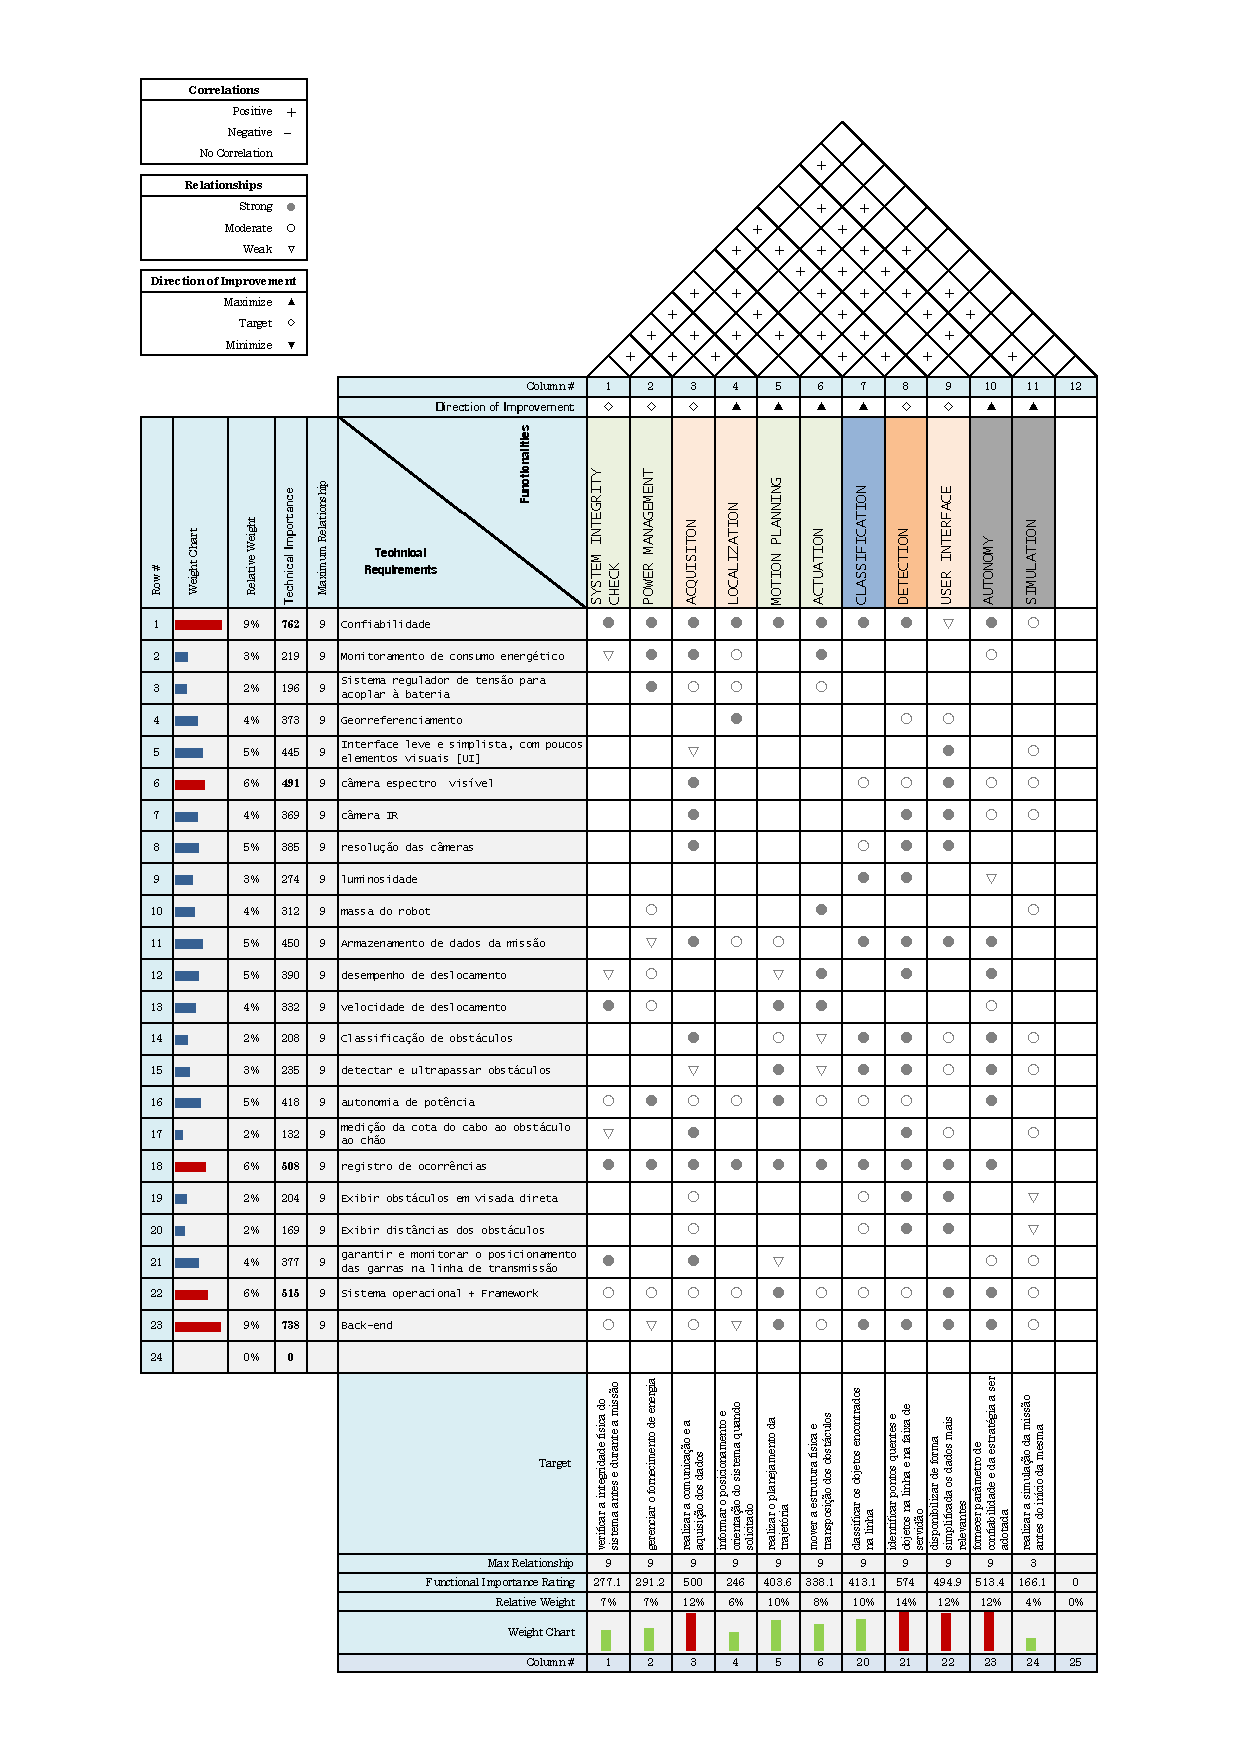
\includegraphics[scale=0.6]{Figures/elirqfd20180710txf.png}
	\end{center}
	\caption{Desdobramento da Função Qualidade - segundo ciclo.}
	%\legend{Fonte: \cite[p. 00]{asdkf}}
	\label{fig_qfd2}
\end{figure}

Para mais detalhes quanto aos objetivos e as descrições das funcionalidades, as mesmas estão contidas na secção \ref{sec:espf}; encontra-se também no Apêndice

%--------- NEW SUB SECTION ----------------------
\subsection{Requisitos técnicos}
\label{ssec:reqt}
    Foi determinado pelo cliente os seguintes requisitos técnicos.
\begin{itemize}
	
\item Desempenho de deslocamento: Percorrer 15km por dia
\item Velocidade de deslocamento: Velocidade média sem obstáculos será de 0.5 m/s
\item Ultrapassagem de obstáculos: Volume máximo dos obstáculos 410x330x150mm
\item Autonomia de Potência: 2 horas de autonomia
\item Sistema Operacional: Linux
\item Backend: C++ e Python
\item Framework: ROS Kinetic Kame

\end{itemize}

\subsubsection{Funcionamento do robô}
O funcionamento do robô será comprovado por um teste realizado dentro da instituição, em um modelo reduzido de linha de transmissão. Sem condições ambientais adversas, realizando a parada baseada no sinal da câmera de detecção de obstáculos e com o teste operado manualmente. Serão desenvolvidas rotinas de software para: início da missão; simular detecção de obstáculo e parada emergencial. As especificações para os testes são:

\begin{itemize}

\item Condutor: LINNET e diâmetro: 18,3mm;
\item Obstáculos: Grampo de suspensão e amortecedor de vibração;
\item O robô será colocado manualmente na linha;
\item A operação se iniciará à uma distância de 1 metro do obstáculo;
\item A parada será realizada com base no sinal do sistema de detecção, a uma distância de 50cm do obstáculo;
\item O comando para início da missão será feito por meio do terminal do Linux , por meio de acesso remoto;
\item A estrutura para o teste será fornecida pela a empresa;

\end{itemize}

As etapas para realização do teste são:

\begin{itemize}
\item O robô será manualmente posicionado na linha, à uma distância de 1 metro do obstáculo;
\item O comando para iniciar a inspeção será enviado via acesso remoto, por meio do terminal Linux;
\item Após receber o comando, o robô iniciará um movimento na linha em direção ao obstáculo;
\item Ao receber o sinal de obstáculo detectado, o robô irá parar e esperar o pós-processamento do sistema de detecção;
\item Após o processamento, irá fazer a ultrapassagem referente ao tipo de obstáculo, e continuar se deslocando na linha;

\end{itemize}

\subsubsection{Códigos da programação disponíveis em repositório online}
Os códigos produzidos serão disponibilizados na plataforma GitHub, onde os pacotes produzidos durante o projeto estão organizados em 4 repositórios referentes às funcionalidades do robô.

\subsubsection{ Documentação técnica de final de projeto}
A documentação foi definida como um relatório denominado Conceptual and Design Report , Databooks com as informações e logbooks com os testes.

\subsubsection{Protótipo do robô}
O cliente disponibilizou as partes mecânicas do robô, sendo entregue pela equipe o protótipo do robô montado. É incluída na montagem a disposição dos cabos e unidade de processamento do robô.


